\begin{figure}[htbp]
\section*{ MPV17}
\centering
\begin{subfigure}[b]{0.95\textwidth}
\centering
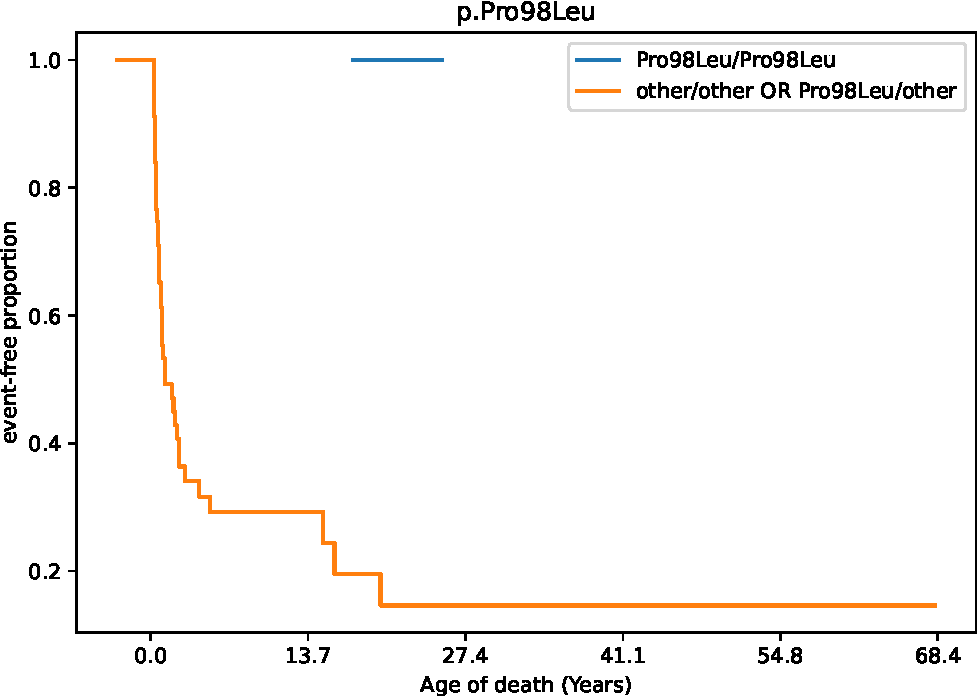
\includegraphics[width=\textwidth]{ img/MPV17_protein_diagram.pdf} 
\captionsetup{justification=raggedright,singlelinecheck=false}
\caption{Distribution of variants in MPV17}
\end{subfigure}

\vspace{2em}

\begin{subfigure}[b]{0.3\textwidth}
\centering
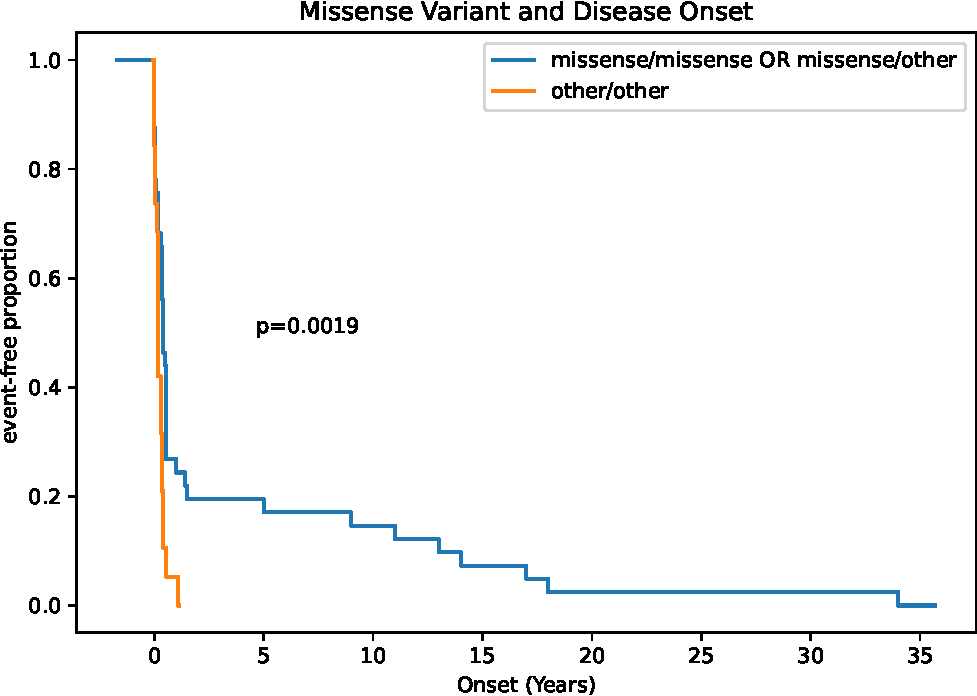
\includegraphics[width=\textwidth]{ img/MPV17_stats.pdf} 
\captionsetup{justification=raggedright,singlelinecheck=false}
\caption{MPV17 disease onset}
\end{subfigure}

\vspace{0.2em}

\begin{subfigure}[b]{0.95\textwidth}
\centering
\resizebox{\textwidth}{!}{
\begin{tabular}{llllrr}
\toprule
HPO term & Pro98Leu/Pro98Leu & other/other OR Pro98Leu/other & p-value & adj. p-value\\
\midrule
Peripheral axonal neuropathy [HP:0003477] & 3/3 (100\%) & 1/22 (5\%) & 0.002 & 0.037\\
\bottomrule
\end{tabular}
}
\captionsetup{justification=raggedright,singlelinecheck=false}
\caption{Fisher Exact Test performed to compare HPO annotation frequency with respect to Pro98Leu/Pro98Leu and other/other OR Pro98Leu/other. Total of
        21 tests were performed. }
\end{subfigure}
\vspace{0.2em}
\begin{subfigure}[b]{0.95\textwidth}
\centering
\resizebox{\textwidth}{!}{
\begin{tabular}{llllrr}
\toprule
Genotype (A) & Genotype (B) & total tests performed & significant results\\
\midrule
missense/missense OR missense/other & other/other & 32 & 0\\
Arg50Gln/Arg50Gln OR Arg50Gln/other & other/other & 29 & 0\\
FEMALE & MALE & 32 & 0\\
\bottomrule
\end{tabular}
}
\captionsetup{justification=raggedright,singlelinecheck=false}
\caption{             Fisher Exact Test performed to compare HPO annotation frequency with respect to genotypes. }
\end{subfigure}

\vspace{0.2em}

\begin{subfigure}[b]{0.95\textwidth}
\captionsetup{justification=raggedright,singlelinecheck=false}
\resizebox{\textwidth}{!}{
\begin{tabular}{llllrr}
\toprule
Description & Variable & Genotype (A) & Genotype (B) & p-value & xrefs\\
\midrule
MTDPS6 (OMIM:256810) age at death & Age of death & Pro98Leu/Pro98Leu & other/other OR Pro98Leu/other & 0.010 & \cite{PMID_20074988,PMID_22593919}\\
\bottomrule
\end{tabular}
}
\caption{ Age of death to compare Pro98Leu/Pro98Leu and other/other OR Pro98Leu/other with respect to Age of death. }
\end{subfigure}

\vspace{0.2em}

\begin{subfigure}[b]{0.95\textwidth}
\captionsetup{justification=raggedright,singlelinecheck=false}
\resizebox{\textwidth}{!}{
\begin{tabular}{llllrr}
\toprule
Description & Variable & Genotype (A) & Genotype (B) & p-value & xrefs\\
\midrule
MTDPS6 (OMIM:256810) disease onset & Onset of OMIM:256810 & missense/missense OR missense/other & other/other & 0.002 & -\\
\bottomrule
\end{tabular}
}
\caption{ Onset of OMIM:256810 to compare missense/missense OR missense/other and other/other with respect to Onset of OMIM:256810. }
\end{subfigure}

\vspace{0.2em}

\caption{ The cohort comprised 60 individuals (30 females, 30 males). 39 of these individuals were reported to be deceased. 
A total of 156 HPO terms were used to annotate the cohort. Disease diagnosis: Mitochondrial DNA depletion syndrome 6 (hepatocerebral type) (MTDPS6; OMIM:256810). 
No clear genotype-phenotype correlation exists. However, a trend for longer survival can be observed in individuals with biallelic pathogenic 
missense variants compared to individuals with biallelic null \cite{PMID_20074988,PMID_22593919}. 
A total of 31 unique variant alleles were found in \textit{MPV17} (transcript: \texttt{NM\_002437.5}, protein id: \texttt{NP\_002428.1}).}
\end{figure}
